%!Mode:: "TeX:UTF-8"
\documentclass[a4paper,11pt,UTF8]{ctexart}

\usepackage{indentfirst} %缩进
\usepackage{xeCJK}    %使用系统字体
\usepackage{fancyhdr} %自定义页眉页脚
\pagestyle{empty}                   %不设置页眉页脚
\usepackage{amsmath, amsthm, amssymb, amsfonts} %数学公式
\usepackage[a4paper,left=3cm,right=3cm,top=3cm,bottom=3cm]{geometry}
%\usepackage[tmargin=1in,bmargin=1in,lmargin=1.25in,rmargin=1.25in]{geometry}.
\usepackage{booktabs} %插入表格
\usepackage[section]{placeins} %避免浮动
\usepackage{listings} %插入代码
\usepackage{ctex}     %中文宏包
\usepackage[svgnames, table]{xcolor} %彩色表格
\usepackage{algorithm}          %伪代码
\usepackage{algorithmicx}
\usepackage{algpseudocode}
\usepackage{algorithm,algpseudocode,float}
\usepackage{lipsum}
\usepackage{enumitem}           %调整列举环境
\usepackage{url}
\usepackage{fontspec,xunicode}
\defaultfontfeatures{Mapping=tex-text} %如果没有它,会有一些 tex 特殊字符无法正常使用,比如连字符。
\usepackage{subcaption}
\usepackage{graphicx}

\graphicspath{{imgs/}}

%%%%%%%%%%%%%%%%%%%%%%%%%%%%%%%%%%%%%%%%%%%%%%%%%%%%%%%%%%%%%%%%
% 缩进及行间距
%%%%%%%%%%%%%%%%%%%%%%%%%%%%%%%%%%%%%%%%%%%%%%%%%%%%%%%%%%%%%%%%
\setlength{\parindent}{22pt} %重新定义缩进长度
\setlength{\baselineskip}{20pt}  %定义行间距
%\renewcommand{\baselinestretch}{1.1} %定义行间距

%%%%%%%%%%%%%%%%%%%%%%%%%%%%%%%%%%%%%%%%%%%%%%%%%%%%%%%%%%%%%%%%
% 列表设置
%%%%%%%%%%%%%%%%%%%%%%%%%%%%%%%%%%%%%%%%%%%%%%%%%%%%%%%%%%%%%%%%
\setenumerate{fullwidth,itemindent=\parindent,listparindent=\parindent,itemsep=0ex,partopsep=0pt,parsep=0ex}
\setenumerate[2]{label=\alph*),leftmargin=1.5em}  %二级item设置
\setitemize{itemindent=38pt,leftmargin=0pt,itemsep=-0.4ex,listparindent=26pt,partopsep=0pt,parsep=0.5ex,topsep=-0.25ex}
\setdescription{itemindent=38pt,leftmargin=0pt,itemsep=-0.4ex,listparindent=26pt,partopsep=0pt,parsep=0.5ex,topsep=-0.25ex}

%%%%%%%%%%%%%%%%%%%%%%%%%%%%%%%%%%%%%%%%%%%%%%%%%%%%%%%%%%%%%%%%
% 图的标题行间距设置
%%%%%%%%%%%%%%%%%%%%%%%%%%%%%%%%%%%%%%%%%%%%%%%%%%%%%%%%%%%%%%%%
\newcommand{\bottomcaption}{%
\setlength{\abovecaptionskip}{6pt}%
\setlength{\belowcaptionskip}{6pt}%
\caption}


%%%%%%%%%%%%%%%%%%%%%%%%%%%%%%%%%%%%%%%%%%%%%%%%%%%%%%%%%%%%%%%%
% 字体定义
%%%%%%%%%%%%%%%%%%%%%%%%%%%%%%%%%%%%%%%%%%%%%%%%%%%%%%%%%%%%%%%%
\setmainfont{Times New Roman}  %默认英文字体.serif是有衬线字体sans serif无衬线字体
\setmonofont{Consolas}
\setCJKmainfont[ItalicFont={楷体}, BoldFont={黑体}]{宋体}%衬线字体 缺省中文字体为
\setCJKsansfont{黑体}
\punctstyle{hangmobanjiao}
%-----------------------xeCJK下设置中文字体------------------------------%
\setCJKfamilyfont{song}{SimSun}                             %宋体 song
\newcommand{\song}{\CJKfamily{song}}
\setCJKfamilyfont{fs}{FangSong}                      %仿宋  fs
\newcommand{\fs}{\CJKfamily{fs}}
\setCJKfamilyfont{ktgb}{KaiTi}                      %楷体2312 ktgb
\newcommand{\ktgb}{\CJKfamily{ktgb}}
\setCJKfamilyfont{yh}{Microsoft YaHei}                    %微软雅黑 yh
\newcommand{\yh}{\CJKfamily{yh}}
\setCJKfamilyfont{hei}{SimHei}                              %黑体  hei
\newcommand{\hei}{\CJKfamily{hei}}
\setCJKfamilyfont{hwxk}{STXingkai}                                %华文行楷  hwxk
\newcommand{\hwxk}{\CJKfamily{hwxk}}
%------------------------------设置字体大小------------------------%
\newcommand{\shiyanbaogao}{\fontsize{36pt}{\baselineskip}\selectfont}
\newcommand{\chuhao}{\fontsize{42pt}{\baselineskip}\selectfont}     %初号
\newcommand{\xiaochuhao}{\fontsize{36pt}{\baselineskip}\selectfont} %小初号
\newcommand{\yihao}{\fontsize{28pt}{\baselineskip}\selectfont}      %一号
\newcommand{\erhao}{\fontsize{21pt}{\baselineskip}\selectfont}      %二号
\newcommand{\xiaoerhao}{\fontsize{18pt}{\baselineskip}\selectfont}  %小二号
\newcommand{\sanhao}{\fontsize{15.75pt}{\baselineskip}\selectfont}  %三号
\newcommand{\sihao}{\fontsize{14pt}{\baselineskip}\selectfont}       %四号
\newcommand{\xiaosihao}{\fontsize{12pt}{\baselineskip}\selectfont}  %小四号
\newcommand{\wuhao}{\fontsize{10.5pt}{\baselineskip}\selectfont}    %五号
\newcommand{\xiaowuhao}{\fontsize{9pt}{\baselineskip}\selectfont}   %小五号
\newcommand{\liuhao}{\fontsize{7.875pt}{\baselineskip}\selectfont}  %六号
\newcommand{\qihao}{\fontsize{5.25pt}{\baselineskip}\selectfont}    %七号

%%%%%%%%%%%%%%%%%%%%%%%%%%%%%%%%%%%%%%%%%%%%%%%%%%%%%%%%%%%%%%%%
% 图题字体大小相同
%%%%%%%%%%%%%%%%%%%%%%%%%%%%%%%%%%%%%%%%%%%%%%%%%%%%%%%%%%%%%%%%
\usepackage{caption}
\captionsetup{font={footnotesize}}   % footnotesize = 9pt
\captionsetup[lstlisting]{font={footnotesize}}

%%%%%%%%%%%%%%%%%%%%%%%%%%%%%%%%%%%%%%%%%%%%%%%%%%%%%%%%%%%%%%%%
% 重定义枚举编号为 1),2)...
%%%%%%%%%%%%%%%%%%%%%%%%%%%%%%%%%%%%%%%%%%%%%%%%%%%%%%%%%%%%%%%%
\renewcommand{\labelenumi}{\theenumi}


%%%%%%%%%%%%%%%%%%%%%%%%%%%%%%%%%%%%%%%%%%%%%%%%%%%%%%%%%%%%%%%%
% 重定义section标题
%%%%%%%%%%%%%%%%%%%%%%%%%%%%%%%%%%%%%%%%%%%%%%%%%%%%%%%%%%%%%%%%
\CTEXsetup[format={\sihao\CJKfamily{zhhei}\zihao{4}},number={\chinese{section}},name={,、~},aftername={},indent={0pt},beforeskip={6pt},afterskip={6pt},format+={\flushleft}]{section}
\CTEXsetup[number={\chinese{section}},name={附录, ~~ }]{appendix}



%%%%%%%%%%%%%%%%%%%%%%%%%%%%%%%%%%%%%%%%%%%%%%%%%%%%%%%%%%%%%%%%
% 标题名称中文化
%%%%%%%%%%%%%%%%%%%%%%%%%%%%%%%%%%%%%%%%%%%%%%%%%%%%%%%%%%%%%%%%
\renewcommand\figurename{\hei 图}
\renewcommand\tablename{\hei 表}
\renewcommand\lstlistingname{\hei 代码}
\renewcommand{\algorithmicrequire}{\textbf{输入:}}
\renewcommand{\algorithmicensure}{\textbf{输出:}}
\newtheorem{define}{定义}

%%%%%%%%%%%%%%%%%%%%%%%%%%%%%%%%%%%%%%%%%%%%%%%%%%%%%%%%%%%%%%%%
% 代码设置
%%%%%%%%%%%%%%%%%%%%%%%%%%%%%%%%%%%%%%%%%%%%%%%%%%%%%%%%%%%%%%%%
\lstset{
 columns=fixed,
 numbers=left,                                        % 在左侧显示行号
 numberstyle=\tiny\color{gray},                       % 设定行号格式
 frame=single,                                        % 单线背景边框
 breaklines=true,                                     % 设定LaTeX对过长的代码行进行自动换行
 keywordstyle=\color[RGB]{40,40,255},                 % 设定关键字颜色
 numberstyle=\footnotesize\color{darkgray},
 commentstyle=\it\color[RGB]{0,96,96},                % 设置代码注释的格式
 stringstyle=\rmfamily\slshape\color[RGB]{128,0,0},   % 设置字符串格式
 showstringspaces=false,                              % 不显示字符串中的空格
 language=java,                                        % 设置语言
 basicstyle=\linespread{1.0}\xiaowuhao\ttfamily,                      % 字体字号
 %lineskip=10pt,
 %baselinestretch=1,
}

%%%%%%%%%%%%%%%%%%%%%%%%%%%%%%%%%%%%%%%%%%%%%%%%%%%%%%%%%%%%%%%%
% 伪代码分页
%%%%%%%%%%%%%%%%%%%%%%%%%%%%%%%%%%%%%%%%%%%%%%%%%%%%%%%%%%%%%%%%
\makeatletter
\renewcommand{\ALG@name}{算法}
\newenvironment{breakablealgorithm}
  {% \begin{breakablealgorithm}
   \begin{center}
     \refstepcounter{algorithm}% New algorithm
     \hrule height.8pt depth0pt \kern2pt% \@fs@pre for \@fs@ruled
     \renewcommand{\caption}[2][\relax]{% Make a new \caption
       {\raggedright\textbf{\ALG@name~\thealgorithm} ##2\par}%
       \ifx\relax##1\relax % #1 is \relax
         \addcontentsline{loa}{algorithm}{\protect\numberline{\thealgorithm}##2}%
       \else % #1 is not \relax
         \addcontentsline{loa}{algorithm}{\protect\numberline{\thealgorithm}##1}%
       \fi
       \kern2pt\hrule\kern2pt
     }
  }{% \end{breakablealgorithm}
     \kern2pt\hrule\relax% \@fs@post for \@fs@ruled
   \end{center}
  }
\makeatother



\begin{document}
\xiaosihao\song

\begin{titlepage}
\center{\yihao{\hwxk{武汉大学国家网络安全学院}}}
\vspace{6cm}
\center{\shiyanbaogao{\ktgb{密~码~学~实~验~报~告}}}
\vspace{4cm}

\begin{center}
\begin{large}
\begin{tabular}{rc}
\xiaoerhao{\hei{学\qquad 号}}& \hspace{1.7cm}\xiaoerhao{\hei{2021302181156\hspace{1.7cm}}} \\
\cline{2-2}\\
\xiaoerhao{\hei{姓\qquad 名}}& \xiaoerhao{\hei{赵~伯~俣}}\\
\cline{2-2}\\
\xiaoerhao{\hei{实验名称}}& \xiaoerhao{\hei{数字签名}}\\
\cline{2-2}\\
\xiaoerhao{\hei{指导教师}}& \xiaoerhao{\hei{何琨}}\\
\cline{2-2}
\end{tabular}
\end{large}
\end{center}
\vfill \hfill
\end{titlepage}
\clearpage

% \centerline{\\[10pt]\erhao{\fs{武 ~汉 ~ 大~ 学}}}
% \centerline{\\[10pt]\yihao{\fs{信~息~隐~藏~实~验~报~告}}}

% \leftline{\\[10pt]\sihao{\hei{\hspace{1.5em} 学生姓名:XXX \hfill 学号:XXXX \hfill 指导教师:XXX }}}

% \leftline{\\[10pt]\sihao{\hei{\hspace{1.5em} 实验地点:新珈楼XXX \hfill }}}

% \leftline{\\[10pt]\sihao{\hei{\hspace{1.5em} 实验时间:第X周周X(X-X节) \hfill }}}



\setlength{\parskip}{6pt}  %定义段间距

\section{实验名称: 数字签名}
\section{实验目的及要求:}
    \subsection{实验目的}
        $(1)$掌握数字签名的概念\par
        $(2)$掌握基于RSA密码、ElGamal密码和椭圆曲线密码的数字签名方法\par
        $(3)$了解基于RSA密码、ElGamal密码和椭圆曲线密码的数字签名的安全性\par
        $(4)$熟悉盲签名的原理,了解盲签名的应用\par

    \subsection{实验要求}
        $(1)$掌握RSA数字签名的实现方案\par
        $(2)$掌握ElGamal数字签名的实现方案\par
        $(3)$掌握SM2椭圆曲线数字签名的实现方案\par
        $(4)$了解数字签名实现中的相关优化算法\par

\section{实验设备环境及要求:}
    Windows操作系统,python高级语言开发环境

\section{实验内容与步骤:}
    \subsection{编程实现RSA数字签名方案}
        \subsubsection{原理}
            设M为明文,$K_{eA}=<e,n>$是A的公钥,$K_{dA}=<d,p,q,\varphi (n)$>是A的私钥,密钥的计算过程在之前的实验中已经实现,在此不过多赘述,
            可以得到用户A对明文M进行签名的过程是\par
            $S_{A}=D(M,K_{dA})=(M^{d}) mod\ n$\par
            计算得到的$S_{A}$便是A对M的签名
            验证签名的过程是\par
            $E(S_{A},K_{eA})=(M^{d})^{e} mod\ n=M$\par
            如果等式成立则签名能够成功验证。

        \subsubsection{实现}
            因为该实验是在上次实验RSA的基础上实现,所以直接调用上次实验的RSA代码。实现代码如下所示
            \lstinputlisting[caption={RSA签名},captionpos=b]{E:/Python_code/codes/cryptography/lab_6/RSA_name/RSA_name.py}

        \subsubsection{思考}
            (1)RSA数字签名方案的几种攻击方法\par
                数学攻击:\par
                    分解法:RSA的安全性基于大数分解的困难。如果攻击者能够分解公钥中的大数(通常是两个大质数的乘积),他们就能破解私钥。
                    这种攻击难度随着所使用的数位长度增加而增加。\par
                    选择密文攻击:攻击者可能会尝试用不同的密文来解密,从而推断出私钥。\par
                实现缺陷攻击:\par
                    侧信道攻击:通过分析硬件实现RSA算法时的物理侧信道信息(如电力消耗、电磁辐射、处理时间等),攻击者可以获得关于私钥的信息。\par
                    错误消息攻击:如果加密系统在处理无效密文时返回的错误消息包含关于密钥的信息,攻击者可能会利用这些信息来推断私钥。\par
                网络攻击:\par
                    中间人攻击:攻击者拦截通信双方之间的消息,伪装成通信的一方向另一方发送消息。在某些情况下,攻击者可能能够替换或篡改数字签名。\par
                    重放攻击:攻击者重新发送或延迟发送合法的数据包,这可能会在没有正确时间戳或序列号的情况下导致安全问题。\par
                协议层面攻击:\par
                    Bleichenbacher攻击:这是对PKCS\#1\ v1.5填充的RSA加密的攻击,它利用了错误格式的RSA密文的错误处理方式来逐渐解密密文。\par

            (2)基于RSA数字签名的盲签名方案的实现\par
                基于RSA数字签名的盲签名方案旨在签名者对信息的内容一无所知。\par
                密钥准备阶段的工作与一般RSA相同,在将所有参数初始化之后进行盲签名过程:\par
                \begin{itemize}
                    \item 盲化消息:
                      \begin{itemize}
                        \item 用户生成随机数 \(r\)(与 \(n\) 互质),计算盲因子 \(b = r^e \mod n\)。
                        \item 用户有消息 \(m\),计算盲化消息 \(m' = m \times b \mod n\)。
                      \end{itemize}
                    \item 请求签名:
                      \begin{itemize}
                        \item 用户将盲化后的消息 \(m'\) 发送给签名者。
                      \end{itemize}
                    \item 签名盲化消息:
                      \begin{itemize}
                        \item 签名者使用私钥 \(d\) 对盲化消息进行签名,计算 \(s' = (m')^d \mod n\)。
                        \item 签名者将签名 \(s'\) 返回给用户。
                      \end{itemize}
                    \item 去盲化:
                      \begin{itemize}
                        \item 用户接收到盲签名 \(s'\),计算真实签名 \(s = s' \times r^{-1} \mod n\)。
                      \end{itemize}
                \end{itemize}
                最后的验证过程可以使用公钥$(e,n)$来计算$S^{e}mod\ n$如果结果等于原始消息m则签名有效
                实现RSA数字签名的盲签名伪代码如下所示
                \begin{algorithm}
                  \caption{RSA盲签名算法}
                  \begin{algorithmic}[1]
                  
                  \Procedure{GenerateKeys}{}
                      \State 生成RSA密钥对 $(e, d, n)$
                      \State \textbf{return} $(e, d, n)$
                  \EndProcedure
                  
                  \Procedure{Blind}{$m, e, n$}
                      \State 选择随机数 $r$,且 $gcd(r, n) = 1$
                      \State 计算盲因子 $b = r^e \mod n$
                      \State 计算盲化消息 $m' = (m \times b) \mod n$
                      \State \textbf{return} $m', r$
                  \EndProcedure
                  
                  \Procedure{Sign}{$m', d, n$}
                      \State 计算盲签名 $s' = (m')^d \mod n$
                      \State \textbf{return} $s'$
                  \EndProcedure
                  
                  \Procedure{Unblind}{$s', r, n$}
                      \State 计算$r$的逆 $r^{-1} \mod n$
                      \State 计算签名 $s = (s' \times r^{-1}) \mod n$
                      \State \textbf{return} $s$
                  \EndProcedure
                  
                  \Procedure{Verify}{$m, s, e, n$}
                      \State 计算 $v = s^e \mod n$
                      \If {$v = m$}
                          \State \textbf{return} True
                      \Else
                          \State \textbf{return} False
                      \EndIf
                  \EndProcedure
                  
                  \end{algorithmic}
                  \end{algorithm}
\newpage                
    \subsection{编程实现ELGamal数字签名方案}
        \subsubsection{复习结论}
          复习数论的一个结论。对于素数q,如果$\alpha $是q的原根,则有:$\alpha ,\alpha ^{2},\dots \alpha ^{q-1}$
          取模(mod q)后各不相同。因此a如果是q的原根,进一步有:\par
          1.对于任意整数m,$\alpha ^{m}\equiv 1(mod\ q)$当且仅当$m\equiv 0(mod\ q-1)$\par
          2.对于任意整数i,j,$\alpha ^{i}\equiv \alpha ^{j}(mod\ q)$当且仅当$i\equiv j(mod\ q-1)$\par
          同ELGamal加密方案一样,ELGamal数字签名方案的基本元素是素数p和$\alpha $,其中$\alpha $是p的原根。
          用户A通过如下步骤产生公钥/私钥对:\par
          1.生成随机整数$X_{A}$使得$1<X_{A}<p-1$\par
          2.计算$Y_{A}=\alpha ^{X_{A}}mod\ p$\par
          A的私钥是$X_{A}$;A的公钥是$\left \{ p,\alpha ,Y_{A} \right \} $
        \subsubsection{原理}
          (1)系统参数:\par
            用户随机地选择一个整数x作为自己的秘密的解密钥,1<x<p-1,计算$y \equiv \alpha ^{x} mod\ p$,
            取y为自己的公开的加密钥。例如选择x=16,$y=\alpha ^{x}mod\ p=10^{16}mod\ 19=4$即私钥为16,公钥为4\par
          (2)产生签名:\par
            将明文消息M(0≤M≤p-1)加密成密文的过程如下:
            \begin{itemize}
              \item 随机地选取一个整数k,k与p-1互素且1≤k≤p-1。例如随机选择k=5
              \item 计算$r=\alpha ^{k}mod\ p=10^{5}mod\ 19=3$\par
                    s=$(m-xr)k^{-1}mod\ p-1=(14-16*3)*5^{-1} mod\ 18=2*11mod\ 18=4$
              \item 取(r,s)=(3,4)作为m=14的签名
            \end{itemize}
          (3)验证签名:\par
            对签名(r ,s)验证的过程如下:
            \begin{itemize}
              \item 计算$V_{1}=\alpha ^{m}mod\ p=10^{14}mod\ 19=16$\par
              \item 计算$V_{2}=y^{r}r^{s}mod\ p=4^{3}*3^{4}mod\ 19=7*5mod\ 19=16$\par
              由于$V_{1}=V_{2}$,所以签名是合法的
            \end{itemize}
            
        \subsubsection{实现}
          实现的ELGamal数字签名程序如下所示
          \lstinputlisting[caption={ELGamal签名},captionpos=b]{E:/Python_code/codes/cryptography/lab_6/ELGamal_name/ELGamal_name.py}

        \subsubsection{例子}
          设p=19,m=14,构造一个ELGamal数字签名方案,并用它对m签名。对于p=19,
          原根有{2,3,10,13,14,15},任选其中之一作为模 19的本原元(生成元),如选择$\alpha $=10
          最终得到的运行结果如下图所示
          \begin{figure}[H]
            \centering
            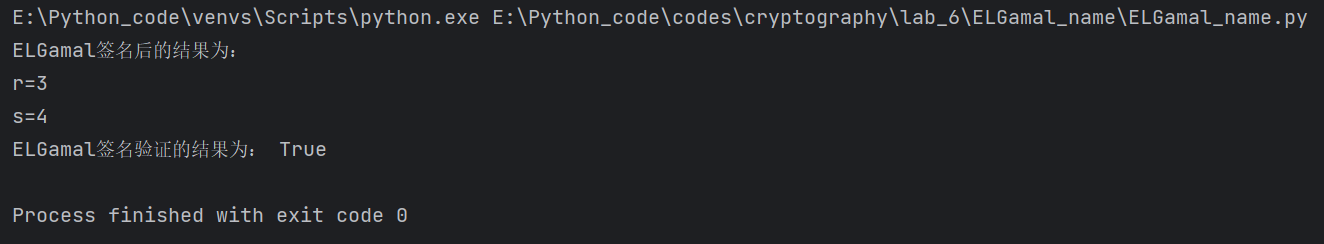
\includegraphics[width=13cm]{ELGamal_result.png}
            \bottomcaption{\xiaowuhao{ELGamal例子处理结果}}
          \end{figure}
        
    \subsection{编程实现SM2椭圆曲线数字签名方案}

        \subsubsection{原理}
          (1)系统参数产生
          \begin{itemize}
            \item 椭圆曲线方程:特定的椭圆曲线方程。
            \item 有限域:椭圆曲线定义在素数域或二元域上。
            \item 基点(G):椭圆曲线上的一个点,其阶为大素数。
            \item 阶(n):基点G的阶,即最小正整数n,使得nG=O(O为无穷远点)。
          \end{itemize}
          (2)产生签名
            \begin{enumerate}
              \item 密钥生成:
              \begin{itemize}
                  \item 随机选择私钥 $d$($1 < d < n$)。
                  \item 计算公钥 $P = dG$。
              \end{itemize}
              \item 生成签名:
              \begin{itemize}
                  \item 随机选择 $k$($1 < k < n$)。
                  \item 计算椭圆曲线点 $(x_1, y_1) = kG$。
                  \item 计算 $r = (e + x_1) \mod n$,其中 $e$ 是消息 $M$ 的哈希值。
                  \item 如果 $r=0$ 或 $r+k=n$,重新选择 $k$。
                  \item 计算 $s = ((1/d) \cdot (k - r \cdot d)) \mod n$。如果 $s=0$,重新选择 $k$。
                  \item 签名为 $(r, s)$。
              \end{itemize}
            \end{enumerate}
          (3)签名验证:
            \begin{enumerate}
              \item 验证 $r$ 和 $s$ 是否在区间 $[1, n-1]$ 内。
              \item 计算消息 $M$ 的哈希值 $e$。
              \item 计算 $t = (r + s) \mod n$。如果 $t=0$,则签名无效。
              \item 计算椭圆曲线点 $(x_1, y_1) = sG + tP$。
              \item 验证 $r$ 是否等于 $(e + x_1) \mod n$。如果等于,则签名有效;否则,无效。
            \end{enumerate}
        \subsubsection{实现}
          实现的SM2签名算法的代码如下所示
          \lstinputlisting[caption={SM2签名},captionpos=b]{E:/Python_code/codes/cryptography/lab_6/SM2_name/SM2_name.py}
        \subsubsection{思考1:椭圆曲线加密、签名的快速实现}
          (1)提示1:模参数、曲线参数的选取优化。选择具有高效运算特性的椭圆曲线,如Koblitz曲线或特定的Weierstrass曲线。
          使用特殊形式的模数,例如梅森素数(Mersenne primes),可以使模运算更快。\par
          (2)提示2:点加和倍点运算的快速实现。例如蒙哥马利梯形算法或双加倍算法。
          使用预计算和窗口方法,预先计算曲线点的多倍数,并在运算时重用这些值。\par
          (3)端到端优化。在硬件层面,使用专门设计的处理器或协处理器来加速椭圆曲线运算。
          在软件层面,使用汇编语言或低级语言优化关键的数学运算,如模乘和模逆。\par
          (4)并行计算。利用现代处理器的多核特性,将一些独立的运算过程并行化。
          对于一些算法步骤,如哈希运算,在多个处理单元上同时执行。\par
          (5)使用特殊的椭圆曲线。例如,Barreto-Naehrig (BN) 曲线可以用于配对加密,
          这些曲线对于特定的密码学应用来说是特别高效的。\par
          (6)减少带宽和存储需求。采用压缩形式的椭圆曲线点表示,只存储和传输x坐标和y坐标的一个位标志,
          从而减少数据的大小。\par

        \subsubsection{思考2:k=15时,kP运算次数}
          反复平方乘 $31P=[11111]2P=2(2(2(2P+P)+P)+P)+P$,共4次加法、4次倍加\par
          改进编码$31P=(25-1)P=2(2(2(2(2P))))-P$,需要5次倍加,1次加法(减法)\par
          因此可以得出在反复平方乘算法中$15P=[1111]2P=2(2(2P+P)+P)+P$共3次加法、3次倍加\par
          改进编码$15P=(16-1)P=2(2(2(2P)))-P$,需要4次倍加,1次加法(减法)\par

\section{实验结果与处理}
  \subsection{RSA数字签名}
    \subsubsection{实验(1)}
      采用上次实验中RSA密码算法的相关参数,对于M进行签名及验证\par
      签名程序运行结果如下图所示
      \begin{figure}[H]
        \centering
        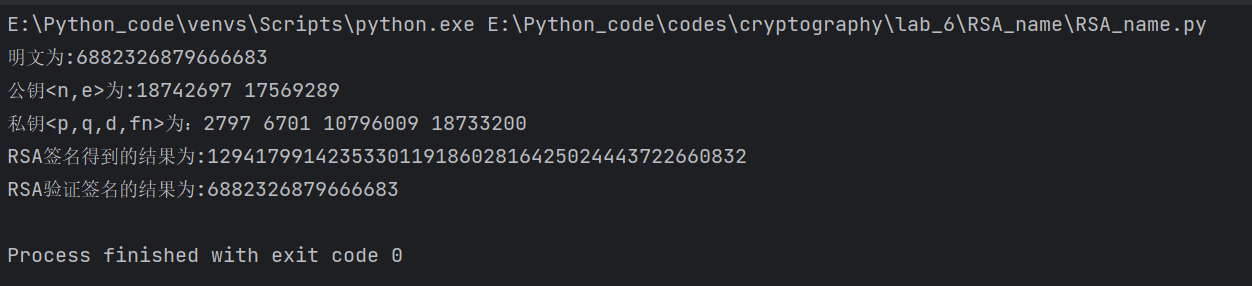
\includegraphics[width=13cm]{RSA_result.png}
        \bottomcaption{\xiaowuhao{RSA运算结果}}
      \end{figure}

  \subsection{ELGamal数字签名}

    \subsubsection{实验(2)}
      采用上次实验中ELGamal密码算法的相关参数对于M进行签名及验证\par
      签名程序运行结果如下图所示
      \begin{figure}[H]
        \centering
        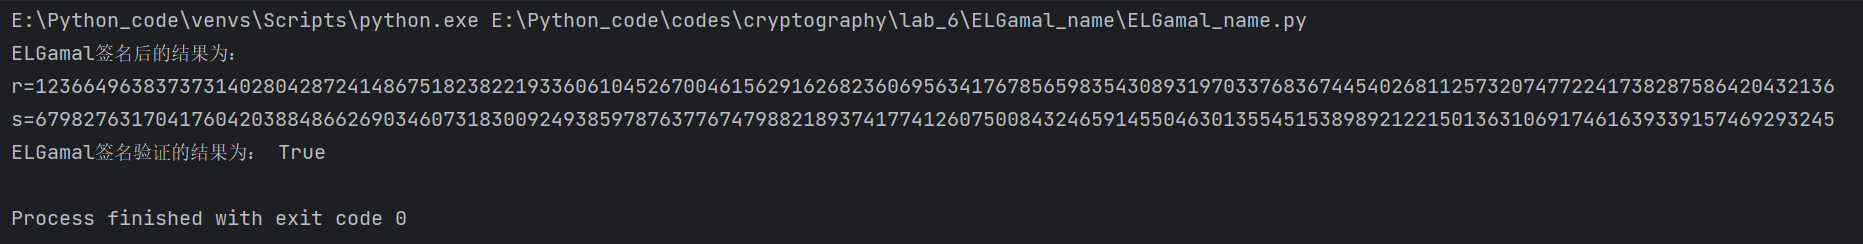
\includegraphics[width=13cm]{ELGamal_result2.png}
        \bottomcaption{\xiaowuhao{ELGamal运算结果}}
      \end{figure}

    \subsubsection{实验(3)}
      任意选作教材p254表8-1中的数字签名的变形算法,对于M进行签名及验证。\par
      选择签名算法为$mx=sk+r mod \ p-1$,选择验证算法为$y^{m}=r^{s}\alpha^{r}mod\ p$\par
      编写验证程序如下所示
      \lstinputlisting[caption={ELGamal变形签名},captionpos=b]{E:/Python_code/codes/cryptography/lab_6/ELGamal_name/ELGamal_name_v2.py}
      该程序的运行结果为
      \begin{figure}[H]
        \centering
        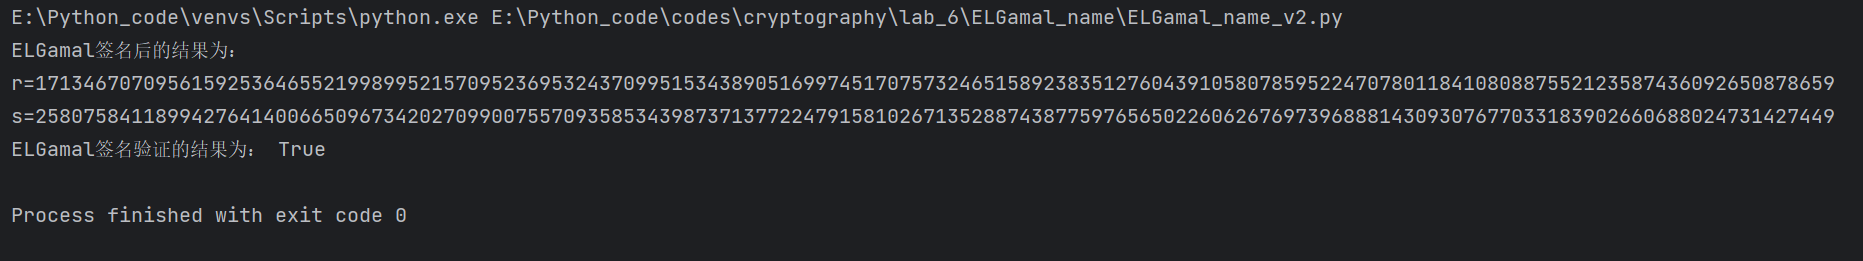
\includegraphics[width=13cm]{ELGamal_result3.png}
        \bottomcaption{\xiaowuhao{ELGamal变形运算结果}}
      \end{figure}
  
    \subsubsection{实验(4)}
      设$r=\alpha ^{k}mod\ p$根据签名算法的一般形式$Ak=B+Cxmod\ p-1$,
      以及对应的验证算法的一般形式$r^{A}=\alpha ^{C}y^{B}mod\ p$,
      自己尝试设计新的基于离散对数的数字签名方案,并对于M进行签名及验证。

  \subsection{SM2数字签名}
      SM2数字签名程序运行结果如下图所示
      \begin{figure}[H]
        \centering
        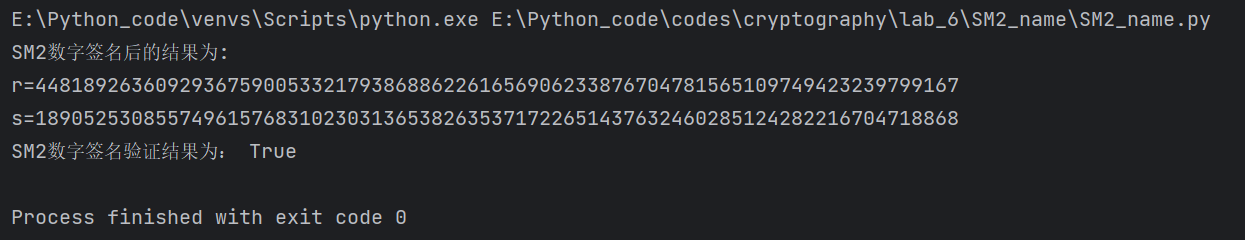
\includegraphics[width=13cm]{SM2_result.png}
        \bottomcaption{\xiaowuhao{SM2运算结果}}
      \end{figure}

\section{分析与讨论}
  通过实践RSA、ElGamal和SM2等不同类型的数字签名方案,我不仅掌握了它们的理论原理,而且对它们在实际应用中的重要性有了更深的理解。
  特别是,我学会了如何在Python环境中实现这些算法,这让我对编程实现密码学算法的过程有了更全面的认识。此外,
  我也对这些算法的安全性有了更深刻的认识,特别是在面对不同类型的攻击时。这次实验不仅增强了我的技术技能,也提高了我的安全意识。


\section{教师评语}

\end{document}
